\documentclass[tikz,border=6pt]{standalone}
\usepackage[T1]{fontenc}
\usepackage[utf8]{inputenc}
\usepackage{amsmath,amssymb}
\usepackage{tikz}
\usetikzlibrary{automata,positioning,arrows.meta,shapes.geometric,calc,fit}
\tikzset{
    >=Stealth,
    every state/.style={minimum size=8mm, inner sep=1pt, font=\small},
    flow/.style={rectangle, rounded corners, draw, align=center, minimum width=3.1cm, minimum height=0.9cm},
    decision/.style={diamond, draw, aspect=2.0, align=center, inner sep=1.5pt},
    terminal/.style={ellipse, draw, align=center, minimum width=2.4cm, minimum height=0.85cm},
    module/.style={rectangle, draw, rounded corners, align=center, minimum width=3.4cm, minimum height=1.0cm},
    data/.style={rectangle, draw, align=center, minimum width=3.2cm, minimum height=0.9cm}
}
\begin{document}
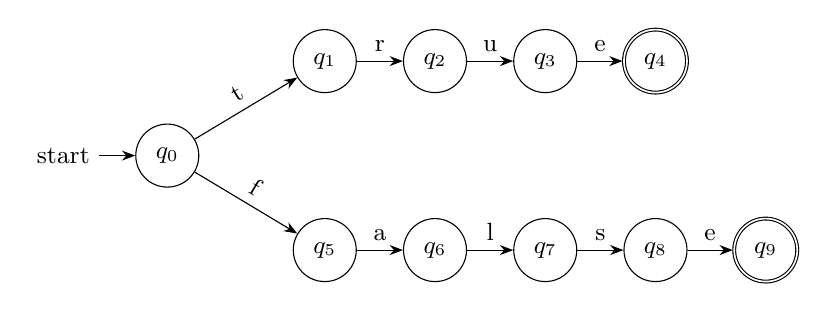
\begin{tikzpicture}[->, font=\small]
    \node[state, initial] (q0) at (0,0) {$q_0$};

    \node[state] (t1) at (2,1.2) {$q_1$};
    \node[state] (t2) at (3.4,1.2) {$q_2$};
    \node[state] (t3) at (4.8,1.2) {$q_3$};
    \node[state, accepting] (t4) at (6.2,1.2) {$q_4$};
    \path (q0) edge node[above,sloped] {t} (t1)
          (t1) edge node[above] {r} (t2)
          (t2) edge node[above] {u} (t3)
          (t3) edge node[above] {e} (t4);

    \node[state] (f1) at (2,-1.2) {$q_5$};
    \node[state] (f2) at (3.4,-1.2) {$q_6$};
    \node[state] (f3) at (4.8,-1.2) {$q_7$};
    \node[state] (f4) at (6.2,-1.2) {$q_8$};
    \node[state, accepting] (f5) at (7.6,-1.2) {$q_9$};
    \path (q0) edge node[above,sloped] {f} (f1)
          (f1) edge node[above] {a} (f2)
          (f2) edge node[above] {l} (f3)
          (f3) edge node[above] {s} (f4)
          (f4) edge node[above] {e} (f5);
\end{tikzpicture}
\end{document}
